\documentclass[solution, letterpaper]{cs121}

\usepackage{graphicx}

%% Please fill in your name and collaboration statement here.
%\newcommand{\studentName}{Renzo Lucioni and Daniel Broudy}
%\newcommand{\collaborationStatement}{I collaborated with...}
\newcommand{\solncolor}{red}
\begin{document}

\header{2}{April 4, 2013, at 11:40 AM}{}{}

%%%%%%%%%%%%%%%%%%%%%%%%%%%%%%%%%%%%%%%%%%%%%%%%%%%%
\section*{Analytical Approach}

\hspace{4mm} The conventional algorithm requires $n^3$ multiplications and $n^2(n-1)$ additions. Thus, the work required by the conventional algorithm, used when $n \leq n_0$, is $n^3 + n^2(n-1) = 2n^3 - n^2$. Strassen's algorithm requires 7 matrix products per recurrence, 10 additions and subtractions when deriving the $P_1, \ldots, P_7$, and 8 additions and subtractions when manipulating the $P_i$'s to find the matrix sums. The work required by Strassen's algorithm, used when $n > n_0$, can be represented by the recurrence $T(n) = 7T(\frac{n}{2}) + (10+8)\frac{n^2}{4} = 7T(\frac{n}{2}) + \frac{9}{2}n^2$, where $T(1) = 1$. Using Mathematica, we find that the solution to this recurrence with the given initial condition is $T(n) = 7^{(\log_2 n) + 1}-6 n^2$. We then simplify this function (so that it clearly agrees with the Big-O running-time for Strassen's of $O(n^{\log_2 7})$) as follows:
\[
\begin{array}{rcl}
T(n) &=& 7^{\log_2 n + 1} - 6n^2\\
&=& 7 \cdot 7^{\log_2 n} - 6n^2\\
&=& 7 \cdot 7^{\frac{\log_7 n}{\log_7 2}} - 6n^2\\
&=& 7 \cdot 7^{\frac{1}{\log_7 2} \cdot \log_7 n} - 6n^2\\
&=& 7 \cdot 7^{\cdot \log_7 n^{\frac{1}{\log_7 2}}} - 6n^2\\
&=& 7 n^{\frac{1}{\log_7 2}} - 6n^2\\
&=& 7 n^{\frac{1}{\frac{\log 2}{\log 7}}} - 6n^2\\
&=& 7 n^{\frac{\log 7}{\log 2}} - 6n^2\\
&=& 7 n^{\log_2 7} - 6n^2\\
\end{array}
\]
This gives us the following function, which we wish to minimize over all $n$:
\[
    f(n)= 
\begin{cases}
    7 n^{\log_2 7} - 6n^2, & \text{if } n > n_0 \\
    2n^3 - n^2, & \text{if } n \leq n_0\\
\end{cases}
\]

We can analytically determine the value of $n_0$ that optimizes the running time of the variant of Strassen's we are studying by setting equal both cases contained in $f$ and solving for $n$. Using Mathematica to solve the equation $7^{(\log_2 n) + 1}-6 n^2 = 2n^3 - n^2$, we see that both sides are equal when $n = 1$ and $n \approx 654.031$. The former value of $n$ is uninteresting, since we already know that the base case of Strassen's algorithm (i.e., when $n=1$) functions the same as the conventional method. Thus, we have analytically determined that $n_0 \approx 654.031$.

\section*{Experimental Approach}

\hspace{4mm}We first implemented both the conventional algorithm for matrix multiplication. We then implemented Strassen's algorithm for matrices where $n$ is a power of 2. We extended this implementation for more general values of $n$ by padding with 0's, as suggested in the hints section of the spec. We tied the two algorithms together by adding a conditional to our implementation of Strassen's to check if the current dimension was less than or equal to the cutoff value; if so, we switch to running our implementation of the conventional algorithm from within Strassen's algorithm. 

We tested for the optimal value of $n_0$ by running our modified version of Strassen's algorithm on matrices where $n=500$ and $n=1000$. In these matrices, every element was randomly selected to be 0, 1, or 2. The graphs below show our results. In the graph for matrices where $n=500$, the compute time is averaged over thirty runs. In the graph for matrices where $n=1000$, the compute time is averaged over fifteen runs.

\begin{center}
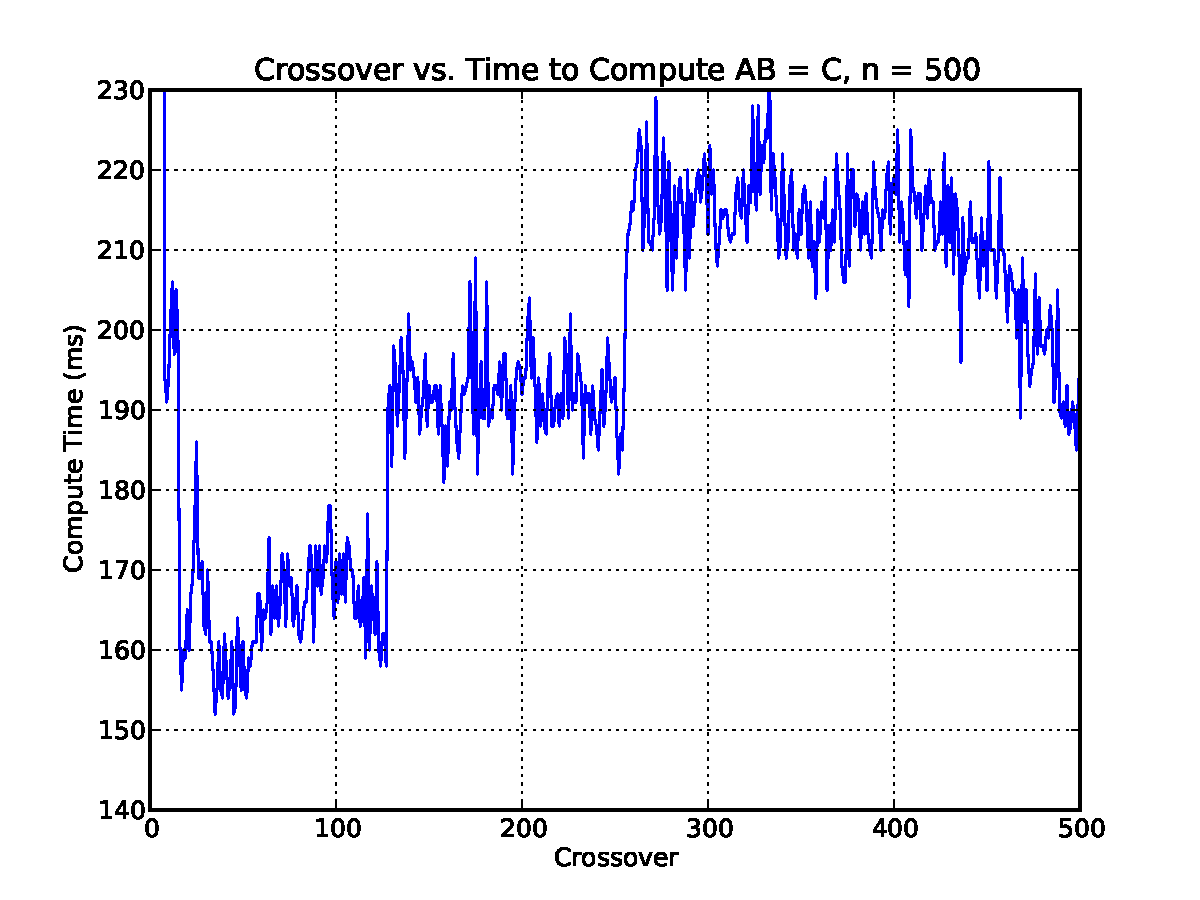
\includegraphics[scale=0.72]{crossover-v-compute-time-500-msec.pdf}
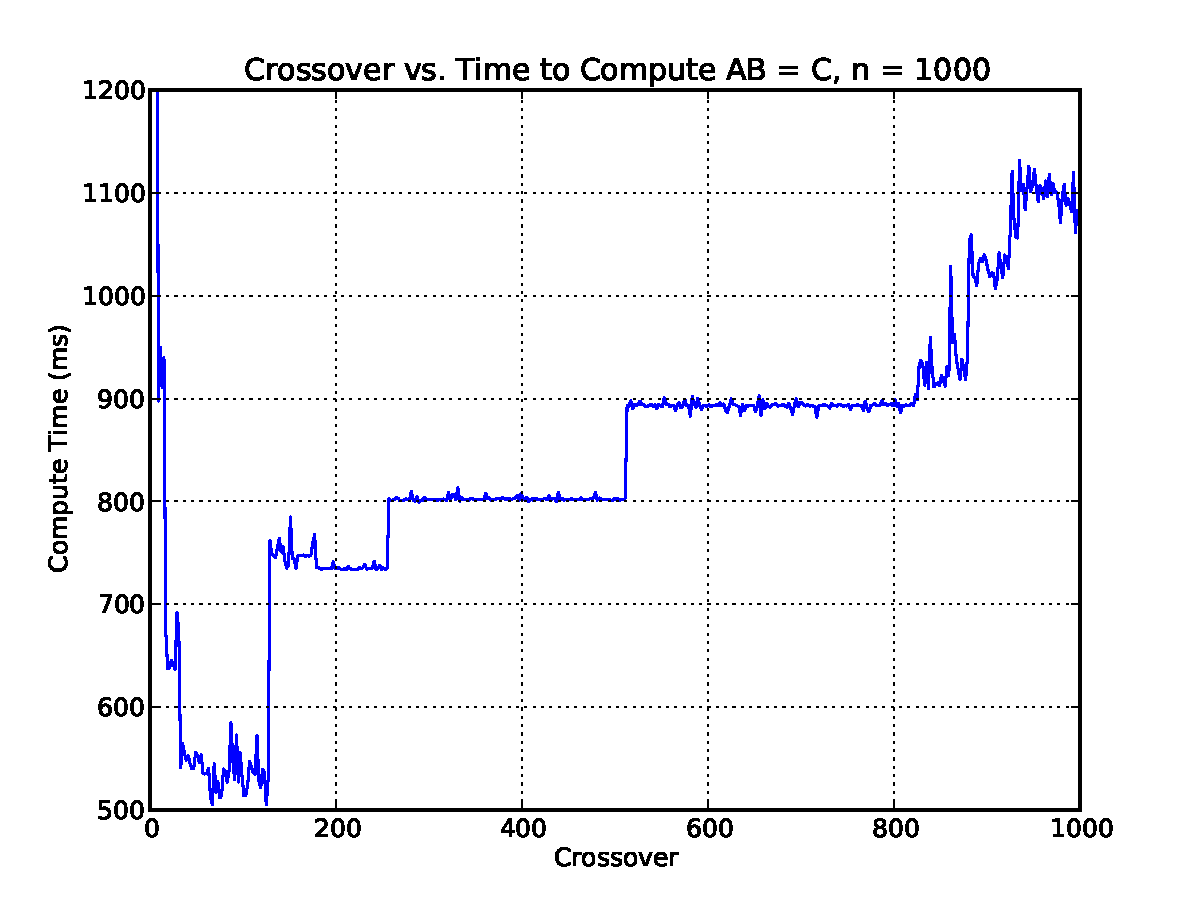
\includegraphics[scale=0.72]{crossover-v-compute-time-1000-msec.pdf}
\end{center}

The stepped pattern in the graphs is immediately clear. Each step corresponds approximately to the nearest power of 2, a side-effect of our padding method (MORE DETAIL), and indicates the time (in microseconds) required to multiply two matrices of the indicated size. In the graph where $n=500$, our minimum compute time, XXX ms, occurs at a crossover of XX. In the graph where $n=1000$, our minimum compute time, 505.27 ms, occurs at a crossover of 34. In both graphs, the lowest step begins near a crossover value of 32, leading us to conclude that in practice, $n_0 = 32$. This cutoff value is now hardcoded into our implementation as a constant; the infrastructure we used to find it is still in place, just commented out. EXPLAIN drop-off at the end?

\section*{Discussion}

\subsection*{Crossover Point}
The lowest crossover point we could decide on was $n_0 = 32$, as discussed above.

\subsection*{Difficulties}
Several difficulties arose when implementing Strassen's.

\subsection*{Optimization}
We sped things up by taking locality of reference into consideration when implementing the conventional algorithm. We applied several optimizations to our implementation of Strassen's.

\subsection*{Largest $n$}
The largest value of $n$ we tested on was $n = 2500$. 

\subsection*{Matrix Type}
In our implementation we chose to multiply {\tt ints}, specifically {\tt int32\_ts}, but this choice does not matter. We could just as easily swap them out for floats, and the program would function as expected.

\end{document}



